%*****************************************
\chapter{Grundlagen}\label{ch:Grundlagen}
%*****************************************
    In den folgenden Abschnitten werden die Grundlagen betrachtet, welche für die Umsetzung eines \ac{IDS} nötig sind.
    Zu Beginn soll in~\autoref{sec:Datenanalyse} geklärt werden welche Analysetechniken für die Überwachung von Systemen zur Verfügung stehen.
    In~\autoref{sec:Datenerfassung} wird dann auf mögliche Orte der Erfassung und in~\autoref{sec:syscalls} auf die eigentliche Daten für die Überwachung, die System Calls, eingegangen.

    Nachdem so eine allgemeine Herangehensweise an die Erkennung von Angriffen dargelegt wurde, 
    soll im Anschluss die Grundlagen des in der Arbeit verwendeten Algorithmus untersucht werden.
    Dazu werden in~\autoref{sec:KNN} \ac{RNN}, sowie die Erweiterung der \ac{RNN}s die \ac{LSTM} neuronalen Netzen beschrieben.

    \section{Intrusion Detection System}\label{sec:IDS}
        Eine \textit{Intrusion} \marginpar{zu dt. Eindringen, Einbruch} ist eine unautorisierte Aktivität welche zu Missbrauch eines Systems führen kann.
        Sie sorgt für ein zum Normalverhalten abweichendes, anormales Verhalten und kann durch diese Abweichung einem System großen Schaden zufügen.
        Ein \ac{IDS} überwacht Ressourcen, wie zum Beispiel Netzwerkdaten und versucht automatisch Missbrauch und anormales Verhalten zu identifizieren, um dadurch die Sicherheit des Systems gewährleisten zu können.~\cite{IDSPIETRO2008}

        Um solche unautorisierten Aktivitäten erkennen zu können müssen Daten erfasst und anschliessend analysiert werden.
        In den folgenden beiden Abschnitten werden verschiedene Ansätze dieser beiden Schritte, also Datenanalyse und Datenerfassung, genauer untersucht.

        \subsection{Datenanalyse}\label{sec:Datenanalyse}
            Das Erkennen von Angriffen auf Computersystemen mittels \ac{IDS} wird im wesentlichen in zwei Kategorien eingeteilt.~\cite{IDSreview, IDSsurvey, IDSsurvey2}.
            Dazu zählen die signaturbasierten und anomaliebasierten Verfahren auf die im Folgenden eingegangen wird.

            \paragraph{Signaturbasiert} 
                \ac{SIDS} versuchen zuvor bekannte Muster von Angriffen in den zu überwachenden Systemen wiederzuerkennen.
                Dies basiert auf einer ausgeprägten Datenbank an Signaturen von bekannten Angriffen.
                Die aktuelle Signatur von zum Beispiel einer Datei wird dann mit Datenbank verglichen.
                Es gibt diverse Möglichkeiten wie diese Signaturen erstellt werden. 
                In mehreren Arbeiten werden dafür zum Beispiel Netzwerk Pakete betrachtet~\cite{IDSsurvey}
                oder auch ein wenig ausgefeilter \textit{State Machines} erstellt~\cite{SIDSstate}\marginpar{zu dt. Zustandsautomaten}.

                \ac{SIDS} haben meist eine sehr hohe Genauigkeit, doch ein wesentlicher Nachteil der signaturbasierten IDS liegt in der Tatsache begründet,
                dass keinerlei neuartigen Angriffe, sowie viele Abwandlungen von schon bekannten Angriffen nicht erkannt werden.
                Das liegt daran, dass für diese Fälle noch keine Signaturen in der Datenbank vorhanden sind.~\cite{IDSPIETRO2008}
                Doch wie in \autoref{sec:einleitung} bereits beschrieben, wird die Gefahr von Zero-Day Angriffen größer als sie bereits ist.
                Weswegen im Folgenden die anomaliebasierte Ermittlung von Intrusions beschrieben wird, die diese Probleme angehen kann.

            \paragraph{Anomaliebasiert}
                Der wesentliche Vorteil Gegenüber den \ac{SIDS} besteht darin, dass auch bisher unbekannte Angriffe erkannt werden können.
                Denn anstatt sich auf bekannte Angriffe zu berufen, werten \ac{AIDS} lediglich eine Abweichung eines wohldefinierten Normalverhaltens als Angriff.
                Das Normalverhalten oder anders formuliert das Modell eines Systems im Normalzustand soll möglichst akkurat das zu erwartende und damit gewollte Systemverhalten beschreiben~\cite{ANOMALYBOOKKISHAN2017}.
                Anomalien oder auch \textit{\glqq outlier\grqq\ }\marginpar{zu dt. Ausreißer} wurden unter anderem schon 1969 definiert.

                \blockquote{An outlying observation, or outlier, is one that appears to deviate markedly from other members of the sample in which it occurs.}~\cite{ANOMALYDEFINITION1969}

                Also eine Anomalie oder wie hier beschrieben eine abweichende Beobachtung, ist eine Beobachtung die deutlich von den anderen Datenpunkten innerhalb der Stichprobe abweicht.
                Anomalien speziell in Daten von Computersystemen können aus verschiedenen Gründen entstehen, zum Beispiel durch böswillige Aktivitäten oder aber auch durch Programmfehler.
                Anomalien dieses Verhaltens können also zu signifikanten und oft kritischen Veränderungen eines Systems führen.
                So kann eine Anomalie in Netzwerkdaten dafür stehen, dass ein gekaperter Computer sensitive Daten an ein unautorisiertes Ziel sendet~\cite{ANOMALYEXAMPLE}.
                Festzuhalten ist also, dass sie das Anomalien eines  Normalverhaltens darstellen und damit interessant für Analysen sind.
                Genau dieser signifikante Unterschied des aktuellen Systemzustand zu einem entworfenen Modell (wohldefiniertes Normalverhalten) zu einem Zeitpunkt $t$ wird dann als Anomalie eingestuft.
                Jede Anomalie gilt dann wiederrum als \textit{Intrusion}.
                Zusammengefasst besteht also die Grundannahme dieser Methode darin, dass Intrusions von dem gelernten Normalverhalten des Systems unterschieden werden können.


                \ac{AIDS} werden im Einsatz in zwei Phasen aufgeteilt, die \textit{Trainingsphase} sowie die \textit{Testphase}.
                Im ersten Schritt der \ac{AIDS} wird ein Modell des Normalverhaltens erstellt.
                Dieser Schritt wird in \ac{ML}-basierte, Statistik-basierte~\cite{IDSPIETRO2008} oder auch 
                wie in manchen Arbeiten~\cite{IDSsurvey} zusätzlich in \textit{Knowledge}-basierten \marginpar{zu dt. Wissens-basierte} Algorithmen untergliedert.
                In der zweiten Phase muss dieses Modell dann überprüft werden.
                Speziell soll dabei mit noch nicht betrachteten Daten getestet werden ob Normalverhalten und Anomalien auch als solche eingestuft werden.
                Dabei liefert der Algorithmus für jede Eingabe entweder einen Anomaliescore oder direkt ein Label\marginpar{Intrusion oder keine Intrusion}.
                Liegt der Score über einem festgelegten Schwellwert so gilt die Eingabe als anormal ansonsten als normal.~\cite{IDSPIETRO2008}

                Jedoch ergibt sich hier im Vergleich zu den \ac{SIDS} eine Problematik.
                Der erwähnte Schwellwert entscheidet über die Ergebnisqualität der \ac{AIDS} und sollte daher sorgfältig und am besten automatisch ermittelt werden, um anwendungsspezifische Justierungen zu vermeiden.\marginpar{mehr dazu in~\autoref{sec:Algorithmus}}

                Die Trainingsphase wird von Chandola et al.~\cite{ANOMALYSURVEY} weiter unterteilt in \textit{Supervised}\marginpar{zu dt. überwacht, unüberwacht},
                \textit{Semi-supervised} sowie \textit{Unsupervised Anomaly Detection}.
                Diese unterscheiden sich hauptsächlich in der Anforderung an die Trainingsdaten. 
                
                Bei einer \textit{Supervised} Anomalieerkennung werden Trainingsdaten verwendet 
                in welchen Anomalien sowie auch Normalverhalten gelabelt sind.
                Somit werden auch Muster von Angriffen gelernt.
                Doch kann es dadurch beim Lernprozess zu Schwierigkeiten kommen, da häufig eine Ungleichgewicht zwischen der Datenmenge an Angriffs- und Normalverhalten besteht.~\cite{IMBALANCEPHUA2004}
                Zusätzlich sind Anomalien meist unbekannt womit das Erstellen eines sinnvollen Datensatzes erschwertwird.
                Auch deswegen ist diese Herangehensweise weniger verbreitet.~\cite{UNSUPERVISEDGOLDSTEIN2016}

                
                Hingegen wird beim \textit{Semi-supervised} Verfahren ein Trainingsdatensatz benötigt welcher lediglich das Normalverhalten kennzeichnet.
                Somit werden auch keine Angriffe zum Trainingszeitraum gesehen.
                Die Grundidee besteht also darin Abweichungen eines Modells des Normalverhaltens zu erkennen.
            
                
                Bei der \textit{Unsupervised Anomaly Detection} werden Daten verwendet welche keine Labels beinhalten.
                Dabei wird davon ausgegangen, dass Normaldaten sehr viel umfangreicher in den Daten vertreten sind als Anomalien.
                Sonst kann es zur Testphase zu häufigen Fehlalarmen kommen, wenn Anomalien fälschlicherweise als Normalverhalten eingestuft werden.~\cite{ANOMALYSURVEY2}.
                Jedoch sind auch \textit{unsupervised} Trainingsverfahren umsetzbar welche keine Anomalien in den Daten enthalten.\cite{UNSUPERVISEDGOLDSTEIN2016}

                Die Wahl des Algorithmus zur Erkennung von Anomalien in den Daten ist dabei entscheidend für den Ablauf der Trainingsphase und wird deshalb auch im Bezug auf das verwendete Verfahren in~\autoref{sec:Training} beschrieben.

                Insgesamt ergeben sich bei der Umsetzung der Anomaliedetektion allerdings auch einige Schwierigkeiten, welche im folgenden zusammengefasst werden:

                \begin{itemize}
                    \item \textit{Definition des Normalverhaltens}:
                        Ziel ist es jegliches Verhalten, welches kein anormales beinhaltet, zu erfassen.
                        So muss dafür gesorgt werden,
                        dass das Normalverhalten auch tatsächlich in den Daten widergespiegelt wird. 

                    \item \textit{Dynamik des Normalverhaltens}:
                        Normalverhalten kann sich über die Zeit verändern 
                        und somit vom Algorithmus Gelerntes unbrauchbar machen~\cite{ANOMALYSURVEY}.

                    \item \textit{Unzulängliche Datensätze}:
                        Daten zur Erfassung des Normalverhaltens sind oft veraltet oder nicht sehr detailreich. 
                        \marginpar{Mehr dazu in \autoref{sec:Datensatz}}

                    \item \textit{Findung eines sinnvollen Schwellwerts}:
                        Festlegung eines Schwellwertes, welcher die eigentliche Unterscheidung zwischen Normalverhalten und Angriffsverhalten umsetzt.
                \end{itemize}

                Die Funktionalität eines \ac{AIDS} steht und fällt also mit den für das Training bereitgestellten Daten.
                % Ist das Normalverhalten im Gänze und in seiner Dynamik richtig dargestellt?
                Daher ist eine entscheidende Frage bei Verwendung von \ac{AIDS}\@: Woher kommen die Daten die für das Training des Normalverhalten benötigt werden.
                Und kann gewährleistet werden, dass diese Daten auch das Normalverhalten genügend präzise beschreiben können.

        \subsection{Datenerfassung}\label{sec:Datenerfassung}
            Die Datenerhebung wird in verschiedenen Arbeiten in zwei Kategorien unterteilt~\cite{IDSsurvey, IDSreview}.
            Zum einen die \ac{HIDS} mit Datenerfassung auf Host-Ebene und zum anderen die \ac{NIDS} bei welchen die Daten auf Netzwerkebene betrachtet werden.
            In den folgenden Abschnitten werden diese beiden Ansätze genauer untersucht.

            \paragraph{Network Based Intrusion Detection}
                Die Grundidee hierbei besteht darin, dass ein Angriff immer den Zugriff auf die Computersysteme von außen erlangen möchte.
                Dafür wird der Netzwerkverkehr über Pakete, NetFlow oder andere Netzwerkdaten überwacht.
                Ein großer Vorteil daran ist, dass viele Computer in einem Netzwerk gleichzeitig überwacht werden.
                Ziel ist es dabei Angriffe möglichst früh zu erkennen und zu verhindern, dass sich die Gefahr weiter ausbreiten kann.
                Die Umsetzung von \ac{NIDS} ist bei besonders großen Netzen erschwert, da der hohe Datendurchsatz das Erkennen von Angriffen erschwert.~\cite{NIDS}

                Ein weiterer Nachteil bei der Untersuchung von Netzwerkpaketen oder ähnlichem besteht darin, dass der Netzwerkverkehr meist verschlüsselt ist und somit nicht auf den Inhalt der Pakete eingegangen werden kann.

            \paragraph{Host Based Intrusion Detection}
                Wie der Name bereits impliziert konzentriert sich \ac{HIDS} auf die Untersuchung von Daten welche auf dem Host basieren.
                Es wird versucht das dynamische Verhalten sowie den Zustand des Systems zu überwachen und dies nur mit Informationen die auf dem Host zugänglich sind.
                In der Literatur werden hierfür verschiedene Informationsquellen genutzt.
                Dazu gehören verschiedene Logs, z.B Firewall und Database Logs~\cite{IDSsurvey},
                oder aber auch Daten aus dem Kernel wie z.B. System Calls~\cite{MAGGI}.
                Im Gegensatz zur \ac{NIDS} kann hier auf den Inhalt von jeder Information eingegangen werden, da die interne Kommunikation unverschlüsselt stattfindet.~\cite{OSSECBRAY2008}

            \paragraph{Host-Daten zur Beschreibung des Systemverhaltens}
                 
                Nach Bridges et al.~\cite{HIDSSURVEY2019bridges} besteht im wesentlichen die Auswahl zwischen Log-Files und \textit{System Calls}\marginpar{zu dt. Systemaufrufe}.
                In der Übersichtsarbeit wird auch noch Literatur besprochen, welche Windows Registry, File System, Programm Analysedaten untersuchen, welche im Folgenden aber nicht mit einbezogen werden.

                Log-Files können weiter aufgeteilt werden in System-Logs und programmspezifischen Logs.
                Wobei System-Logs nur durch das Betriebssystem geschrieben werden.
                Beide Log Arten beschreiben das Systemverhalten jedoch findet bei beiden bereits eine Filterung von Informationen des Normalverhaltens statt.
                Denn es muss manuell bestimmt werden welche Aktionen überhaupt geloggt werden und stellen deshalb auch keine vertrauenswürdige Quelle dar~\cite{SEMANTICSCREECH2014}.
                System Calls hingegen sind klar definiert und beschreiben das Systemverhalten zunächst ungefiltert, unterliegen dafür allerdings einer weitaus größeren Varianz.~\cite{HIDSSURVEY2019bridges}\marginpar{mehr dazu in~\autoref{sec:syscalls}}
                Für die feingranulare Aufzeichnung von Log-Files sowie für System Calls gilt, dass die Aufzeichnung sehr rechenintensiv werden kann.
                Mit modernen Softwarelösungen wie zum Beispiel sysdig~\cite{SYSDIG}, kann der Berechnungsaufwand für viele Anwendungsbereiche in akzeptable Bereiche gebracht werden.
                In dieser Arbeit wird auf die Filterung durch Logs verzichtet und auf die detailliertere Darstellung des Systemverhaltens durch System Calls gesetzt.


                \autoref{fig:IDSOverview} soll einen Überblick über die in den vorigen Abschnitten gemachte Einstufung geben.
                \begin{figure}[ht]
                    \centering
                    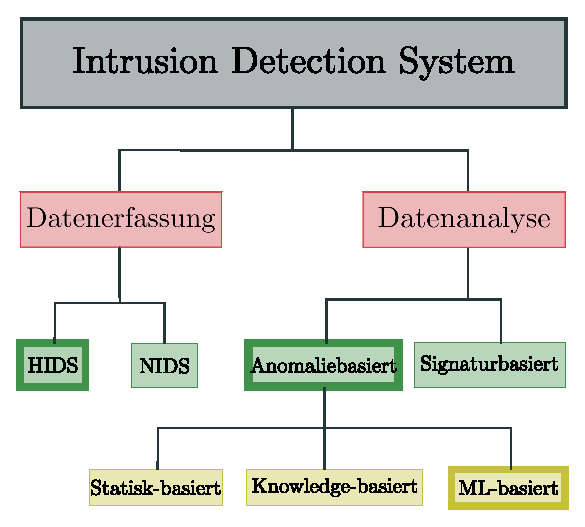
\includegraphics[width=0.7\textwidth]{images/Illustrationen/IDS/IDSOverview}
                    \caption{Einordnung des verwendeten \ac{IDS} (Relevant für diese Arbeit dicker markiert).}\label{fig:IDSOverview}
                \end{figure}
                Dabei gibt die Abbildung die Strukturierung der vorigen Abschnitte wieder,
                in welcher die Datenerfassung in die Host-basierte und Netzwerk-basierte Erfassung unterteilt wird sowie die Datenanalyse
                in die anomaliebasierten und signaturbasierten Verfahren eingeteilt wird.
                Die dicker umrandeten Verfahren werden in dieser Arbeit verwendet.
                Also zur Datenerfassung werden nur Informationen welche auf dem Host zugänglich sind verwendet 
                und die so erhaltenen Daten werden anomaliebasiert untersucht.
                Es stellen sich beim designen von anomaliebasierten \ac{HIDS} zwei Hauptfragen:
                \begin{itemize}
                    \item Mit welchen Daten kann das Systemverhalten möglichst präzise dargestellt werden?
                        \begin{itemize}
                            \item Logs, System Calls, Registry \dots~\cite{HIDSSURVEY2019bridges}
                        \end{itemize}
                    \item Wie wird die eigentliche Anomalie in den Daten erkannt?
                \end{itemize}
                Die letztere Frage soll speziell in~\autoref{sec:Algorithmus} beleuchtet werden, doch wie das Systemverhalten präzise dargestellt werden kann soll nun behandelt werden.
                In dieser Arbeit werden System Calls als Beschreibung des Systemverhalten verwendet.
                Im Folgenden sollen Grundlagen der System Calls besprochen werden.
                Zusätzlich soll untersucht werden welche Informationen neben der eigentlichen Sequenz der System Calls zur Verfügung stehen.

    \section{System Calls}\label{sec:syscalls}
        Jegliche Programme die auf einem Rechner mit einem Betriebssystem laufen, müssen mit diesem interagieren um Veränderungen am System vornehmen zu können.
        Diese Interaktion findet in Form von \textit{System Calls}\marginpar{zu dt. Systemaufrufe} statt und kann mit einem gewöhnlichen \ac{API} verglichen werden.
        Beispielhaft werden in \autoref{tab:syscall} zwei System Calls von Linux Betriebssystemen, ihre Argumente und die Art ihrer Rückgabewerte beschrieben.

        \begin{table}[ht]
            \small
            \centering
            \begin{tabular}{cp{4cm}p{2cm}p{3cm}}
                \hline
                \rowcolor{GruvGray!36}
                \multicolumn{4}{c}{System Calls}\\
                \hline
                Name & Beschreibung & Argumente & Rückgabewerte\\
                \hline
                \hline
                \rowcolor{GruvGray!16}
                %open& Öffnet die von \textit{pathname} spezifizierte File. Falls diese nicht existiert kann sie mit dem Zusatz \textit{O_CREAT} automatisch erstellt werden & path, asdklfjs, slddk\\
                open& Öffnet die in \textit{path} spezifizierte File und gibt einen \textit{file descriptor} zurück.& \textit{path}, \textit{flags}, \textit{mode} & File descriptor oder Fehlerwert\\
                write& Schreibt bis zu \textit{count} Bytes aus dem Buffer (ab Stelle \textit{buf}) in die File, welche über den \textit{file descriptor}$fd$ definiert wird. & $fd$, $*buf$, \textit{count} & Geschriebene Bytes oder Fehlerwert\\
                \hline
            \end{tabular}
            \caption{Kurzbeschreibung ausgewählter System Calls}
            \label{tab:syscall}
        \end{table}

        \subsection{Allgemeines}

        Generell werden System Calls verwendet um vom Betriebssystem zur Verfügung gestellte Funktionalitäten auszuführen.
        Das Betriebssystem, oder noch genauer der \textit{Kernel} \marginpar{zu dt. Betriebssystemkern} des Betriebssystems stellt verschiedene Services bereit, welche dann von Programmen genutzt werden können. 
        Die System Calls stellen dabei die Kommunikation zwischen dem Kernel und den darauf laufenden Programmen dar.
        Zu den Services gehören verschiedene Bereiche der Prozesskontrolle, das Datei- und Geräte-Management, Informationspflege und Kommunikationsaufbau und zugehörige Aufgaben.
        Geschrieben werden diese Funktionalitäten in C, C++ oder auch in Assembly.
        Üblicherweise können System Calls nur von Nutzerprozessen, also aus dem \textit{User space}\marginpar{zu dt. Benutzer-Modus/Benutzerprozesse}, aufgerufen werden, diese besitzen eine eingeschränkte Berechtigungen.
        In~\autoref{fig:syscallAblauf} wird der Ablauf in welchem ein Programm aus dem User space über einen System Call eine privilegierte Aktion ausführen lassen kann dargestellt.
        Dies ermöglicht es Nutzerprozessen auf eine limitierte Auswahl an privilegierten Funktionen aus dem Kernel zugreifen zu können.~\cite{SYSCALL_SILBERSCHATZ}
    
        \begin{figure}[ht]
            \centering
            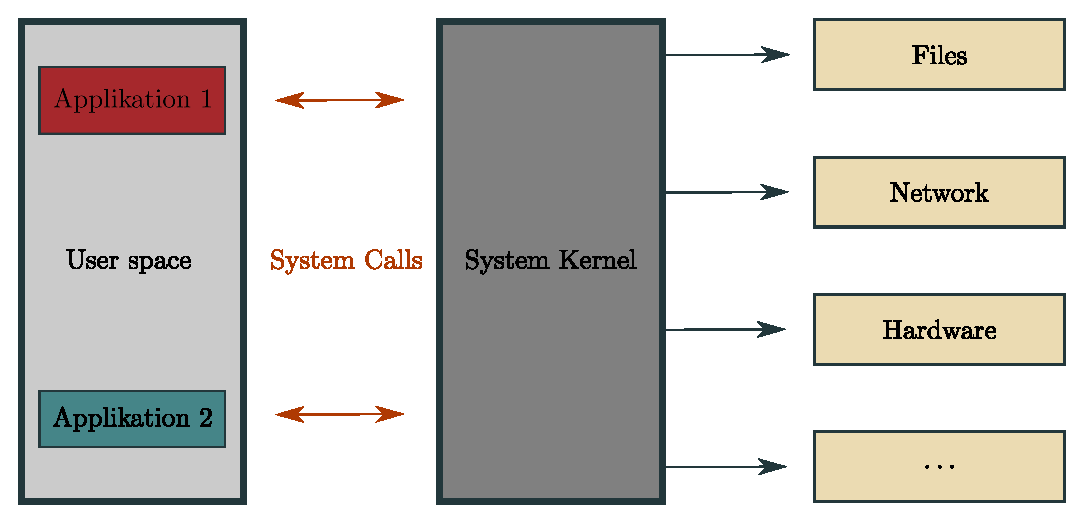
\includegraphics[width=1\textwidth]{images/Illustrationen/IDS/syscalls}
            \caption{Darstellung der Kommunikation zwischen Applikationen aus dem User space mit dem System Kernel und dem Kernel mit Dateien/Netzwerk/Hardware/\dots}
            \label{fig:syscallAblauf}
        \end{figure}

        Wie in~\autoref{fig:syscallAblauf} ebenfalls angedeutet, besteht ein System Call aus einem Aufruf an das Betriebssystem und der Antwort des Betriebssystems.
        In \autoref{tab:syscall} beschrieben besitzen System Calls Argumente die beim Aufrufen mitgegeben werden können.        
        Das können neben bestimmten Flags, welche die Funktion der System Calls bestimmen, auch zum Beispiel Dateipfade oder IP-Adressen sein.~\cite{SYSCALL_MANPAGE}
        Die Betriebssystemantworten auf einen System Calls haben zusätzlich in den Argumenten einen Rückgabewert~\marginpar{Gekennzeichnet mit \glqq $res$\grqq}.
        Zu den Rückgabewerten gehören unter anderem diverse Fehlerwerte, aber auch zum Beispiel bei \textit{read} oder \textit{write} System Calls die Menge an gelesenen oder geschriebenen Bytes.
        Zu einem System Call gehört also mehr als nur der Funktionsname.


        Ein Angreifer muss also um Schaden anzurichten Veränderungen an den System Calls vornehmen.
        Der folgende Abschnitt soll einen Überblick verschaffen, wie die System Calls für ein \ac{IDS} verwendet werden können.
        %Denn eine Veränderung der System Call Sequenz kann auch verhindert werden.

        \subsection{System Calls für IDS}
            Viele verschiedene \ac{IDS} Ansätze betrachten die Sequenz von System Calls und erzielen vielversprechende Ergebnisse.~\cite{MAGGI}
            Häufig werden dabei aber nicht die in den Argumente der System Calls enthaltene Information mit einbezogen und bieten damit einen Spielraum für Angriffe.
            Verschiedene Arbeiten~\cite{Syscallseqexploit1, Syscallseqexploit2, Syscallseqexploit3} zeigen, wie dieser Spielraum ausgenutzt werden kann um unerkannt Angriffe durchzuführen. 
            Tan et al.~\cite{Syscallseqexploit3} erreichen dies durch die Veränderung eines zuvor von der \ac{IDS} erkannten Angriffes.
            % Sie beschreiben wie sie dem \ac{IDS} unbekannte System Call Sequenzen präsentierenI@derart Verändert werden können, dass sie als normal eingestuft werden.
            Dabei werden die dem \ac{IDS} fremden Sequenzen auseinander gezogen und mit bekannten Sequenzen aufgefüllt.\marginpar{Verwendeter Algorithmus: STIDE~\cite{FORREST}} 
            Ein weiterer Ansatz versucht lediglich die System Call Argumente zu verändern, ohne dabei die Sequenz zu beeinflussen~\cite{Syscallseqexploit1}.
            Was diese Beispiele jedoch zeigen, ist dass wenigstens einer dieser Faktoren, also entweder die Sequenz von System Calls verändert werden muss oder es werden die Argumente der System Calls verändert.
            So könnte zum Beispiel anstatt auf den Pfad \glqq /tmp/some/file\grqq \ auf \glqq /etc/passwd\grqq \ zugegriffen werden. 
            Welche dieser Argumente und wie diese genutzt werden können um die Anomalieerkennung zu verbessern soll in \autoref{sec:Meta} untersucht werden.
            In dem nachfolgenden Kapitel wird nun auf verschiedene Datensätze, welche System Call Sequenzen und teilweise Argumente und weiter Metadaten enthalten, eingegangen.

        \subsection{Datensätze}\label{sec:Datensatz}
            Seit 1998 einer der ersten System Call Datensätze für \ac{HIDS} veröffentlicht wurde~\cite{DARPA, KDD},
            kamen über die Jahre verschiedene weitere Datensätze hinzu.
            Auf diese wird in den kommenden Abschnitten kurz eingegangen.
            Dabei soll auch auf die Nutzbarkeit und die entstehenden Problematiken dieser für die \ac{HIDS} über System Calls eingegangen werden.
            \paragraph{DARPA}
                Der unter anderen von der \textit{Defence Advanced Research Project Agency}, kurz DARPA, erstellte Datensatz KDD-99~\cite{DARPA} lieferte einen der ersten Benchmark Datensätze für \ac{HIDS}.
                Er simuliert ein militärisches Netzwerk bestehend aus drei Systemen mit unterschiedlichen Betriebssystemen und Services.
                Diese Systeme erzeugen mit wechselnden IP-Adressen Traffic, welcher insgesamt fünf Wochen über TCP-Dump aufgezeichnet wurde.
                Dabei werden verschiedene Angriffe ausgeführt, darunter sind \textit{Denial of Service} und \textit{User to Root}\marginpar{Auch als \textit{Priviledge Escalation} bezeichnet}.
                Der Datensatz steht auf Grund verschiedener Unzulänglichkeiten schon länger in der Kritik~\cite{KDDCRITIC, UNM, KDDCRITIC2}.
                Unter anderem beschreiben McHugh et al.~\cite{KDDMCHUGH}, dass eine Unausgewogenheit zwischen Angriffs- und Normaldaten bestehen.
                Zum Beispiel gibt es Aufnahmetage, an welchen bis zu 76\% der Daten Angriffsdaten entsprechen, was laut McHugh keine realistische Verteilung ist.
                Eine der größten Kritikpunkte, welcher auch von Tavallaee et al.~\cite{KDDCRITIC2} und Engen~\cite{ENGEN2010} aufgefasst wird, besteht in der Redundanz der Aufnahmen.
                So haben Tavallaee et al.\ alle mehrfach vorkommenden Aufnahmen entfernt und damit 78.05\% der Trainingsdaten und 17.15\% der Testdaten entfernt.
                Gerade bei selbstlernenden Systeme kann dadurch ein ungewollter Bias entstehen.
                Des Weiteren ist der Datensatz mittlerweile stark veraltet (1999/1998).
            \paragraph{UNM}
                Der \textit{University of New Mexico} Datensatz stammt aus dem Jahr 2004 und beinhaltet die Aufzeichnung von System Calls diverser Programme, welche alle Administratorenrechte besitzen.
                Dabei wurden verschiedene Angriffe, wie zum Beispiel \textit{Buffer  Overflows} ausgeführt.
                Auch dieser Datensatz~\cite{UNM} ist mittlerweile veraltet und kommt für eine weitere Betrachtung nicht in Frage,
                da er zusätzlich auch keine weiteren Kontextinformationen wie Thread IDs enthält~\cite{UNMcritic}.
            \paragraph{ADFA-LD}
                Der \ac{ADFA-LD} wurde von Creech et al.~\cite{UNMcritic} im Jahre 2013 erstellt und ist damit wesentlich aktueller als die zuvor genannten.
                Dieser wurde auf einem Linuxsystem aufgezeichnet, dessen Schwachstellen von verschiedenen \textit{Penetration Testing} Tools ausgenutzt werden.
                Aufzeichnungen wurden auf dem Betriebssystem Ubuntu 11.04 durchgeführt, allerdings wurden diese nicht gut dokumentiert was ein Bearbeiten erschwert~\cite{ADFA-LDcritic}.
                Hinzu kommt, dass lediglich Sequenzen von System Call IDs aufgezeichnet wurden und damit keine Metadaten im Datensatz enthalten sind.
            \paragraph{NGIDS-DS}
                Der 2017 erstellte Datensatz NGIDS \cite{NGIDS} wurde mit Hilfe der dedizierten Security Hardware \textit{IXIA Perfect Storm} aufgezeichnet.
                Er beinhaltet Thread Informationen, aber auch hier fehlen weitere Daten wie zum Beispiel System Call Argumente.
                Ein weiteres großes Problem liegt in der Ungenauigkeit der Zeitstempel, welche nur auf die Sekunde genau sind und es ergeben sich Schwierigkeiten in der Zuordnung der beschriebenen Event ID und den Zeitstempeln~\cite{LIDDS}.
            \paragraph{LID-DS}
                2019 veröffentlichten Grimmer et al.~\cite{LIDDS} das \textit{Leipzig Intrusion Detection-Data Set} (LID-DS).
                Sie erkannten, dass die bisherigen Datensätze entweder veraltet oder nicht ausreichend waren um zum Beispiel Thread IDs oder System Call Argumente für ein \ac{IDS} zu verwenden.
                Er wurde auf einem modernen Betriebssystem Ubuntu 18.04 aufgenommen und besteht aus 10 verschiedenen Szenarien auf welchen jeweils ein Angriff ausgeführt wird.
                Jedes Szenario repräsentiert damit also eine bekannte Schwachstelle eines Systems.
                In~\autoref{tab:scenarien} werden die verschiedenen Schwachstellen als \ac{CVE}
                \marginpar{zu dt. Allgemeine Schwachstellen und Gefährdungen} oder \ac{CWE} \marginpar{zu dt. Aufzählung gemeinsamer Schwachstellen} bezeichnet.
                CVE ist ein Industriestandard der für eine einheitliche Namenskonvention für Sicherheitslücken verwendet wird.
                Bei den CWEs handelt es sich um eine von der Community gepflegte und von der MITRE Corporation veröffentlichte Auflistung verschiedener Typen von Schwachstellen in Soft- und Hardware.
                Aufgezeichnet werden für jedes Szenario neben den Namen der System Calls auch deren Metadaten.
                Dazu zählen unter anderem die Parameter, Rückgabewerte, Zeitstempel sowie User-, Prozess- und Thread-IDs.
                %{\color{red}Für die spätere Suche nach sinnvollen zusätzlichen Informationen eines System Calls lohnt es sich hier ein wenig detaillierter auf die in \autoref{tab:scenarien} beschriebenen Szenarien zu schauen.
                %Auffällig ist zunächst das Bruteforce-CWE-307 Szenario.
                %Dabei wird ein Bruteforce Angriff durchgeführt in welchem in kurzer Zeit diverse Anmeldeveruche stattfinden.
                %Hier unterscheiden sich die Abläufe der System Calls zwischen Normal- und Angriffsverhalten unter anderem durch die auftretende Frequenz.
                %Ein weiterer spannen
                %Return Values}
                \begin{table}[]
                    \scriptsize
                    \centering
                    \begin{tabular}{p{3cm}p{6.5cm}}
                        \rowcolor{GruvGray!36}
                        \hline
                        \multicolumn{2}{c}{Szenarien}\\
                        \hline
                        \thead{Name} & \thead{Beschreibung} \\
                        \rowcolor{GruvGray!16}
                        \hline
                        \hline
                        Bruteforce-CWE-307 & \makecell[l]{\textbf{Setup:} Simple Wordpress Web-Applikation \\ \textbf{Schwachstelle:} Ungeeignete Einschränkung von \\übermäßigen Authentifizierungsversuchen} \\
                        \hline
                        CVE-2012-2122 & \makecell[l]{\textbf{Setup:} Oracle MySQL Datenbank \\ \textbf{Schwachstelle:} Mehrfacher falscher Loginversuch \\führt zu erfolgreichem Login} \\
                        \rowcolor{GruvGray!16}
                        \hline
                        CVE-2014-0160 & \makecell[l]{\textbf{Setup:} Simple Web-Applikation \\ \textbf{Schwachstelle:} Fehler in OpenSSL Implementierung,\\ Heartbleed} \\
                        \hline
                        CVE-2017-7529 & \makecell[l]{\textbf{Setup:} Nginx Web-Applikation \\ \textbf{Schwachstelle:} Datenleck durch \textit{Integer Overflow} } \\
                        \rowcolor{GruvGray!16}
                        \hline
                        CVE-2018-3760 & \makecell[l]{\textbf{Setup:} Rails Web-Applikation \\ \textbf{Schwachstelle:} Informationsleck durch \textit{Sprockets}} \\ 
                        \hline
                        CVE-2019-5418 & \makecell[l]{\textbf{Setup:} Rails Web-Applikation \\ \textbf{Schwachstelle:} Schwachstelle in Applikations-\\Controller} \\
                        \rowcolor{GruvGray!16}
                        \hline
                        EPS\_CWE-434 & \makecell[l]{\textbf{Setup:} Upload Service\\ \textbf{Schwachstelle:} Keine Upload-Beschränkungen} \\
                        \hline
                        PHP\_CWE-434 & \makecell[l]{\textbf{Setup:} Web-Applikation \\ \textbf{Schwachstelle:} Keine Upload-Beschränkungen} \\
                        \rowcolor{GruvGray!16}
                        \hline
                        SQL Injection & \makecell[l]{\textbf{Setup:} Web-Applikation mit SQL-Datenbank \\ \textbf{Schwachstelle:} SQL-Injection} \\
                        \hline
                        ZipSlip & \makecell[l]{\textbf{Setup:} Uploading Portal für Zip Dateien\\ \textbf{Schwachstelle:} Dateien werden ohne Überprüfung \\ dekomprimiert} \\
                        \hline
                    \end{tabular}
                    \caption{Kurzbeschreibung der in dem Datensatz vorkommenden Szenarien und den dazugehörigen Sicherheitslücken~\cite{LIDDS}}
                    \label{tab:scenarien}
                \end{table}

                Jedes Szenario beinhaltet insgesamt ca. 1000 30-60 Sekunden lange Aufzeichnungen.
                Die ersten 200 Aufzeichnungen dienen als Trainingsdaten, die darauffolgenden 50 als Validierungsdaten und die restlichen als Testdaten. 
                Dabei sind mindestens in 100 Aufzeichnungen der Testdaten Angriffe enthalten, für welche der Angriffszeitpunkt gegeben ist.
                Jede dieser Aufzeichnungen ist in einer Datei gespeichert, welche in einer $runs.csv$ beschrieben und zusammengefasst werden.
                 
                In~\autoref{tab:runsfile} wird ein Ausschnitt aus der beschreibenen $runs.csv$ dargestellt und in~\autoref{tab:syscallfile} eine Beispieldatei einer tatsächliche Aufzeichnung von System Calls.
                \begin{table}[ht]
                    \small
                    \centering
                    \begin{tabular}{l | g | l}
                        \rowcolor{GruvGray!36}
                        \hline
                        \multicolumn{3}{c}{runs.csv}\\
                        \hline
                        \hline
                        \rowcolor{White}
                        Eintrag & Beispieldatei 1 & Beispieldatei 2 \\
                        \hline
                        image\_name& file\_1 & file\_2\\
                        scenario\_name& scenario\_1 & scenario\_1 \\
                        is\_executing\_exploit& False & True \\
                        warmup\_time& 10 & 10 \\
                        recording\_time& 53 & 40 \\
                        exploit\_start\_time &-1 & 15\\
                    \end{tabular}
                    \caption{Ausschnitt aus der runs.csv des LID-DS, welche unter anderem die Labels für Angriffsfiles und Normalfiles enthalten.~\cite{LIDDS}}
                    \label{tab:runsfile}
                \end{table}
                \begin{table}[ht]
                    \scriptsize
                    \centering
                    \begin{tabular}{l || g | l | g}
                        \rowcolor{GruvGray!36}
                        \hline
                        \multicolumn{4}{c}{System Call}\\
                        \hline
                        \rowcolor{White}
                        Eintrag & System Call 1 & &System Call x \\
                        \hline
                        evtent number & 26 & & 4012 \\
                        evtent time &$11:09:47.592865922$ & & $10:18:20.1231231231$ \\
                        user uid & 101 & & 33 \\
                        process name & nginx &\dots & apache2 \\
                        thread id & 21822 & & 1425 \\
                        evtent dir & < & & > \\
                        evtent type & sendfile & & writev \\
                        evtent args & $res=612$, $offset=1225$ & &\makecell{$fd=12(<4t>172.131.12.1:123 \\ \rightarrow172.13.231.2:123)$, $size=2392$} \\
                        \hline
                    \end{tabular}
                    \caption{Ausschnitt aus den eigentlichen Aufzeichnungen von System Calls aus dem LID-DS~\cite{LIDDS}}
                    \label{tab:syscallfile}
                \end{table}
                \paragraph{Problem des LID-DS}

                    In den Testdaten mit enthaltenen Angriffen wird ein Angriffszeitpunkt angegeben.
                    Jedoch gibt es bei einer Datei mit Angriff im Gegensatz zu den normalen Dateien vier statt zwei mögliche Zuordnungen.
                    In den normalen sind das zum einen \ac{TN}, falls kein Alarm vorliegt, da in den normalen Dateien keine Angriffe stattfinden.
                    Oder falls fälschlicherweise ein Angriff erkannt wird, die Zuordnung als \ac{FP}.
                    Die Zuordnungen der Dateien mit Angriff werden in~\autoref{fig:quadrant} dargestellt.
            
                    \begin{figure}[ht]
                        \centering
                        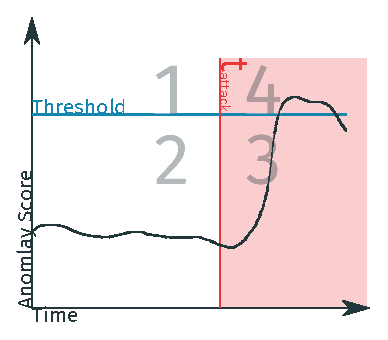
\includegraphics[width=0.8\textwidth]{images/q_problem.eps}
                        \caption{Illustration des Quadrantenproblems (inspiriert von~\cite{IDSTHREADGRIMMER2021}).
                        Es beschreibt die Problematik, dass Alle System Calls nach $t_{Angriff}$ als bösartig eingestuft werden müssen, obwohl auch Normalverhalten stattfindet.}
                        \label{fig:quadrant}
                    \end{figure}

                    Befindet sich der Anomaliescore vor dem Angriffszeitpunkt $t_{Angriff}$ unter dem Schwellwert, also im Quadrant 3 der Abbildung, kann von einem \ac{TN} ausgegangen werden.
                    Also es wurde korrekterweise kein Alarm vorhergesagt.
                    Befindet sich der Anomaliescore vor dem Angriffszeitpunkt $t_{Angriff}$ über dem Schwellwert, also im Quadrant 2, liegt ein \ac{FP} vor.
                    Es wurde ein Alarm gemeldet an einer Stelle an dem (noch) kein Angriff stattfand.
                    Nach dem angegebenen Angriffszeitpunkt $t_{Angriff}$ wird es allerdings schwieriger.
                    Denn liegt der Anomaliescore nach dem Angriffszeitpunkt über dem Schwellwert, also im Quadranten 1, wird von einem \ac{TP}, also einem korrektem Alarm ausgegangen.
                    Jedoch könnte der Angriff zu diesem Zeitpunkt schon vorbei sein.
                    Also könnte ein Alarm nach $t_{Angriff}$ theoretisch auch ein \ac{FP} sein. 
                    Genauso könnte umgekehrt ein Anomaliescore unter dem Schwellwert, also im Quadranten 4 korrekt sein obwohl er als \ac{FN} gewertet werden müsste.
                    Diese Problematik wird auch von Grimmer et al.~\cite{IDSTHREADGRIMMER2021} aufgegriffen und muss in der Auswertung beachtet werden. 
                    In~\autoref{sec:Metriken} wird eine Lösungsmöglichkeit für die Problemstellung betrachtet.


                Nachdem nun verschiedene allgemeine Ansätze zur Erkennung von schädlichem Verhalten eines Systems und mögliche Datensätze zur Auswertung untersucht wurden,
                soll im Folgenden die Frage geklärt werden, wie mit Hilfe von künstlichen neuronalen Netzen Muster in einem Datensatz erkannt werden können.

    \section{Künstliche neuronale Netze}\label{sec:KNN}        
        Das Übertragen von bestehenden und in der Natur vorkommenden Strukturen und Prozessen kommt in verschiedenen Forschungsbereichen zum Einsatz.
        Auch zum Beispiel in direkter Umsetzung für Oberflächenstrukturen welche häufig in der Raumfahrt eingesetzt werden~\cite{GECKO}, oder auch Abstrakter in der Umsetzung von Verhaltensweisen von Ameisen~\cite{ANT}.
        Ein in den letzten Jahren immer weiter verbreiteter Ansatz in der elektronischen Datenverarbeitung ist die Verwendung von künstlichen neuronalen Netzen.
        Diese haben Neuronen und neuronale Netze als biologisches Vorbild.
        Dabei ist allerdings die abstrakte Modellierung der Informationsverarbeitung im Vordergrund und nicht das Nachbilden der biologischen neuronalen Netze.
        Man verspricht sich mit dem Einsatz von künstlichen neuronalen Netzen, welche eine Varietät an verschiedenen Architekturen beinhalten, diverse Optimierungsprobleme zu lösen.
        %In dieser Arbeit wird der Einsatz von neuronalen Netzen zur \textit{Time Series Prediction} (zu dt. Vorhersagen von Zeitreihen) untersucht.
        Zu aktuellen Beispielen zählen dabei auch Vorhersagen die im Zusammenhang mit der Verbreitung des COVID-19 Virus stehen~\cite{COVID1, COVID2, COVID3}.
        %Für die \textit{Time Series Prediction} sind verschieden Architekturen von neuronalen Netzen weit verbreitet \cite{BENIDIS2020}.
        
        Algorithmen in welchen neuronale Netze zum Einsatz kommen bestehen generell aus zwei Phasen. 
        In der ersten Phase, der Trainingsphase, werden vordefinierte Trainingsdaten in das Netz gegeben.
        Dieses versucht Merkmale in den Daten zu ermitteln, mit welchen dann in der Testphase Voraussagen gemacht werden können.
        Dabei haben sich spezialisierte Herangehensweisen entwickelt, wie zum Beispiel die \ac{CNN} für die Bilderkennung. 
        Für sequentielle Daten wie Audio, Text und Video, bei welchen eine zeitliche Komponente entscheidend ist, eignen sich vor allem die \ac{RNN}.
        Da in dieser Arbeit sequentielle Daten betrachtet werden, die sequentielle Abfolge von System Calls, soll im Folgenden nur auf die \ac{RNN} und eine besondere Abwandlungen dieser eingegangen werden.
        % überarbeiten
        %unterteilung verschiedener Netze und einordnung von rnns und lstmnn
        %Neuronale Netze bestehen aus verschiedenen Ebenen von Knoten (auch Neuronen genannt), die miteinander verbunden sind.
        %Die Neuronen erhalten Eingangssignale und falls diese eine bestimmte Bedingung erfüllen (z.B. Schwellwertüberschreitung) wird das Ausgangssignal des Neurons verändert.
        %Wird die Bedingung nicht erfüllt, sendet das Neuron ein Signal, welches die nachfolgenden Neuronen nicht beeinflusst. Der schematische Aufbau wird in Abbildung \ref{fig:Neuron} gezeigt.
        \subsection{Rekurrente neuronale Netze}\label{sec:RNN}
            Der entscheidende Unterschied von RNNs zu herkömmlichen neuronalen Netzen ist,
            dass der Ausgang eines Knotens auf einer \textit{Layer} \marginpar{zu dt. Ebene} mit einer vorherigen oder derselben Layer verbunden ist.
            Ist dies der Fall spricht man von einem \textit{Feedback} oder \textit{Recurrent Neural Network}, sonst von einem \textit{Feedforward Neural Network}. 
            Mit Knoten, die eine extra Verbindung zu sich selbst haben, können frühere Eingaben Einfluss auf die Behandlung der nächsten Eingabe haben.
            Der einzelne Knoten merkt sich seine Ausgabe, welche im nächsten Zeitschritt als weiteres Eingabesignal dient.
            Dadurch wird es ermöglicht auch zeitlich abhängige Sequenzen zu erlernen, da die Signalverarbeitung der RNNs auch vorherige Geschehnisse mit einbezieht.
            Im Gegensatz dazu steht zum Beispiel die Bilderkennung, bei welchem das vorherige Bild keinen Einfluss auf die Einschätzung des aktuellen Bildes hat.
            Dieser Zusammenhang lässt sich in der folgenden Gleichung darstellen.
            \begin{equation}
                \begin{split}
                    h_t &= \sigma \left(W_{h}h_{t-1} + W_{x}x_{t} + b\right)\\
                    y_t &= h_t
                \end{split}
            \end{equation}
            Dabei beschreiben $x_t$, $h_t$ und $y_t$ den Eingang des Neurons, die rekurrente Information und den Ausgang des RNN\@.
            $W_h$ und  $W_x$ beschreiben die Gewichte und $b$ den Bias.
            Ein einzelner Knoten wird ohne die Gewichte in~\autoref{fig:RNN} dargestellt,
            sowie in~\autoref{fig:RNN_enroled} in einer alternativen Darstellung, wie sich dieser Knoten $A$ über $t$ Zeitpunkte verhält.
            Dabei werden für die Übersichtlichkeit Gewichte sowie der Bias nicht dargestellt.
                \begin{figure}[ht]
                    \centering
                    \includegraphics[width=0.8\textwidth]{images/Illustrationen/RNN_simple}
                    \caption{Darstellung einer RNN Zelle}
                    \label{fig:RNN}
                \end{figure}
                \begin{figure}[ht]
                    \centering
                    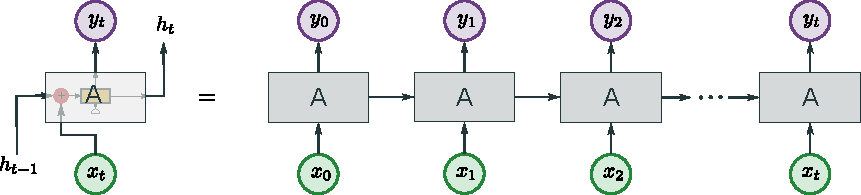
\includegraphics[width=1\textwidth]{images/Illustrationen/RNN_enrolled}
                    \caption{Darstellung einer \glqq ausgerollten\grqq \ und vereinfachten RNN Zelle}
                    \label{fig:RNN_enroled}
                \end{figure}
            Doch auch die RNNs haben ein Problem bei Merkmalen, die sich über einen längeren Zeitraum strecken.
            Denn dabei kommt es häufig vor, dass durch die \textit{Backpropagation} die berechneten Gradienten entweder verschwindend klein, oder sehr groß werden.
            Gerade bei Abhängigkeiten über einen größeren zeitlichen Abstand tendieren die Fehlersignale,
            die durch die Backpropagation durch das Netz gegeben werden, zu geringe Gewichtsänderungen auszulösen.
            Traditionelle Aktivierungsfunktionen wie die hyperbolische Tangensfunktion haben Gradienten im Bereich $(-1,1)$ oder $[0,1)$ und Backpropagation berechnet Gradienten durch die Kettenregel.
            Dies hat den Effekt, dass n dieser kleinen Zahlen multipliziert werden, um die Gradienten der \glqq vorderen\grqq \ Schichten in einem n-Schichten-Netzwerk zu berechnen, was bedeutet, dass der Gradient (Fehlersignal) exponentiell mit n abnimmt und die vorderen Schichten sehr langsam trainieren.
            Die von Sepp Hochreiter erstmals erwähnte \textit{Long Short-Term Memory} (LSTM) Zellen ermöglichen durch verbesserte Fehlerkorrektur stabilere Lernergebnisse sowie auch das Lernen von Mustern mit noch größeren zeitlichen Abständen.~\cite{HOCHREITER1998}

            Diese Sonderform der RNNs, die auch in dieser Arbeit verwendet werden, sollen deshalb genauer untersucht werden.
            %% TODO Batch Normalisation \cite{LSTMbatchnorm}
   	
        \subsection{Long Short-Term Memory} 
            Hauptziel der \acp{LSTM} ist es, das Lernen der zeitlich abhängigen Muster zu verbessern.
            Entscheidend dafür ist die Einschätzung welche zuvor gesehenen Informationen für die aktuelle Eingabe relevant sein könnten.
            
            \begin{figure}[ht]
                \centering
                \includegraphics[width=1\textwidth]{images/Illustrationen/LSTM}
                \caption{Schematische Darstellung eine Memory Cell $A$ in einem LSTM NN, mit Input, Output und Forget Gate (inspiriert von \cite{OLAH2015}).}
                \label{fig:LSTM}
            \end{figure}

            Und um zu erlernen welche früheren Ausgaben für die Ermittlung nächster Datenpunkte entscheidend sind,
            wird an jedem Knoten eine mit $A$ in der~\autoref{fig:LSTM} gekennzeichnete \textit{Memory Cell} \marginpar{zu dt. Gedächtniszelle} angebracht.
            Sie ist mit sich selbst verbunden, kennt also die vorherigen Ausgaben und gibt den Zellstatus an.
            Mit Hilfe dieser Information soll eine Abhängigkeit auch über einen längeren Zeitraum gefunden werden.
            Der Zellstatus $C_{t-1}$ zum Zeitpunkt $t-1$ hat im nächsten Zeitschritt $t$ einen Einfluss auf den Zellstatus $C_{t}$ und somit auch auf die Ausgabe $y_t$.
            Die Weitergabe des Status wird in~\autoref{fig:LSTM_Status} dargestellt.

                \begin{figure}[ht]
                    \centering
                    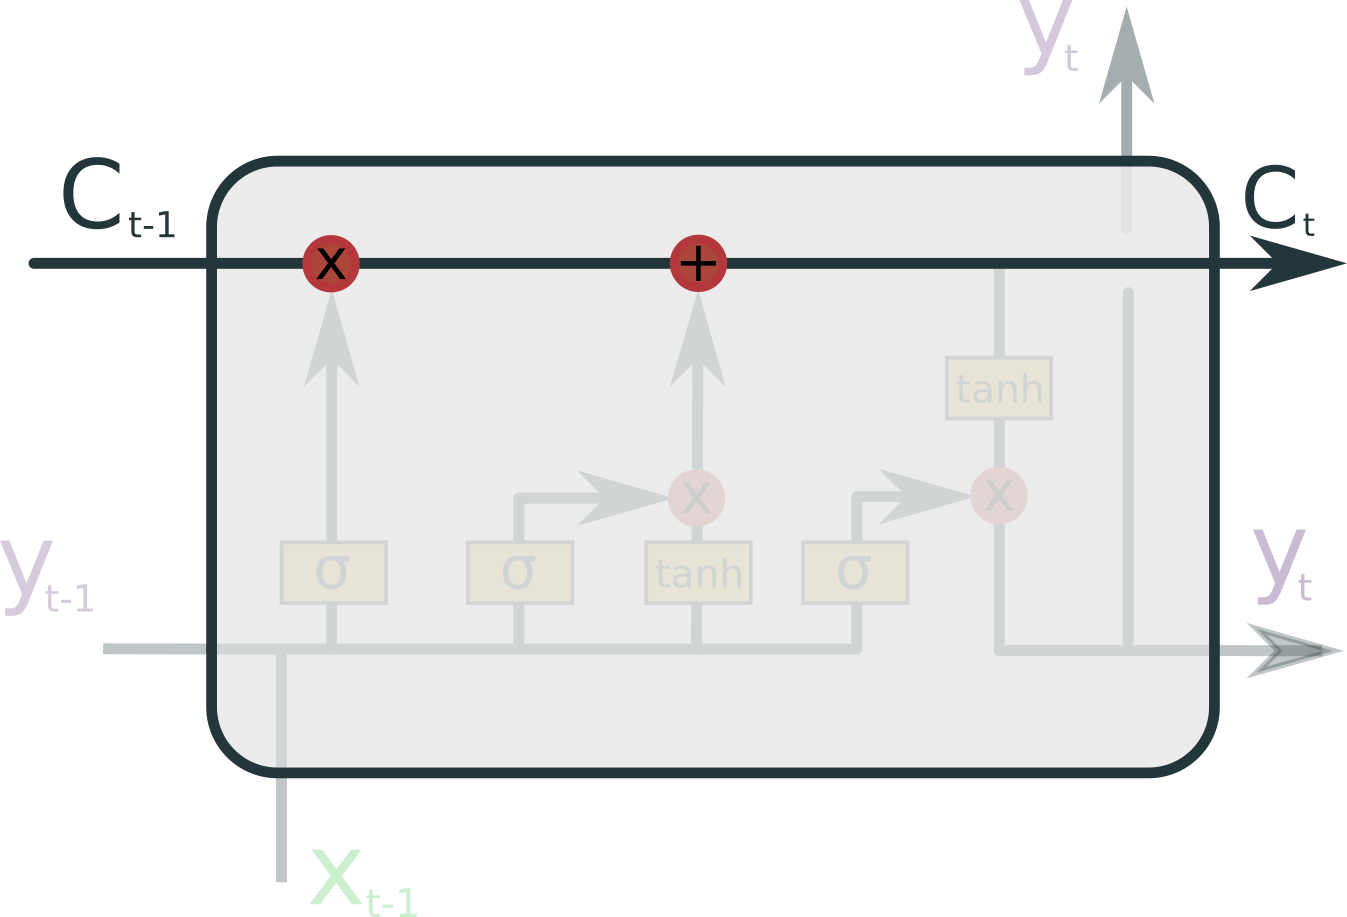
\includegraphics[width=0.5\textwidth]{images/Illustrationen/LSTM_MC}
                    \caption{Weitergabe des Zellstatus innerhalb eines Knotens (inspiriert von \cite{OLAH2015}).}
                    \label{fig:LSTM_Status}
                \end{figure}
                
                Einfluss auf den Zellstatus haben zwei verschiedene \textit{Gates} \marginpar{zu dt. Gatter/Tore}.
            Im ersten Schritt wird entschieden, welche Information aus dem vorherigen Zeitschritt keinen Einfluss mehr auf den Zellstatus haben sollen.
            Dies wird mit dem \textit{Forget Gate} umgesetzt und ist in~\autoref{fig:LSTM_Forget} zu sehen und kann analog zur RNN Zelle folgendermaßen hergeleitet werden.

            \begin{equation}
                f_t = \sigma\left(W_{fh}h_{t-1} + W_{fx}x_t + b_f\right)
            \end{equation}

            $W_{fh}$ und $W_{fx}$ beschreiben die Gewichte $b_f$ den Bias des \textit{Forget Gate}.
            Es wird also die vorherige Eingabe $h_{t-1}$ sowie die aktuelle Eingabe $x_t$ gewichtet und mit Bias an die Aktivierungsfunktion $\sigma$ übergeben.
            Damit sollen Informationen aus dem Speicher, die keinen Einfluss mehr haben sollen, entfernt werden.
            In dem Sprachbeispiel könnte das Genus (\textit{grammatikalisches Geschlecht}) gespeichert werden, um so eine grammatikalisch korrekte Vorhersage zu machen.
            Kommt nun allerdings ein neues Pronomen in der Eingabe $x_t$, sollte das bisher gespeicherte Genus keinen Einfluss mehr haben.
            
                \begin{figure}[ht]
                    \centering
                    \includegraphics[width=0.5\textwidth]{images/Illustrationen/LSTM_FG}
                    \caption{Einfluss des Forget Gates auf den Zellstatus (inspiriert von \cite{OLAH2015}).}
                    \label{fig:LSTM_Forget}
                \end{figure}
                
            Das \textit{Input Gate} soll im nächsten Schritt angeben, welche neuen Informationen in den Zellstatus $C_t$ aufgenommen werden.
            Dies erfolgt in zwei Schritten, zunächst wird mit $i_t$ ermittelt, welche Information geupdated werden soll.

            \begin{equation}
                \begin{split}
                    i_t &= \sigma\left(W_{ih}h_{t-1} + W_{ix}x_t + b_i\right), \\
                    \tilde{C}_t &= tanh\left(W_{\tilde{C}h}h_{t-1} + W_{\tilde{C}x}x_t + b_{\tilde{C}}\right),\\
                \end{split}
            \end{equation}

            Im Vektor $\tilde{C}$ sind mögliche Kandidaten enthalten (wie z.B. das Genus), welcher den zuvor vergessenen Wert ersetzen soll (vgl.~\autoref{fig:LSTM_Input}).
            Der gesamte Zellstatus $C_t$ wird dann zusammen mit Werten aus dem \textit{Forget Get} verrechnet.

            \begin{equation}
                \begin{split}
                    C_t &=f_t\times C_{t-1} + i_t\times \tilde{C}_t, \\
                \end{split}
            \end{equation}

                \begin{figure}[ht]
                    \centering
                    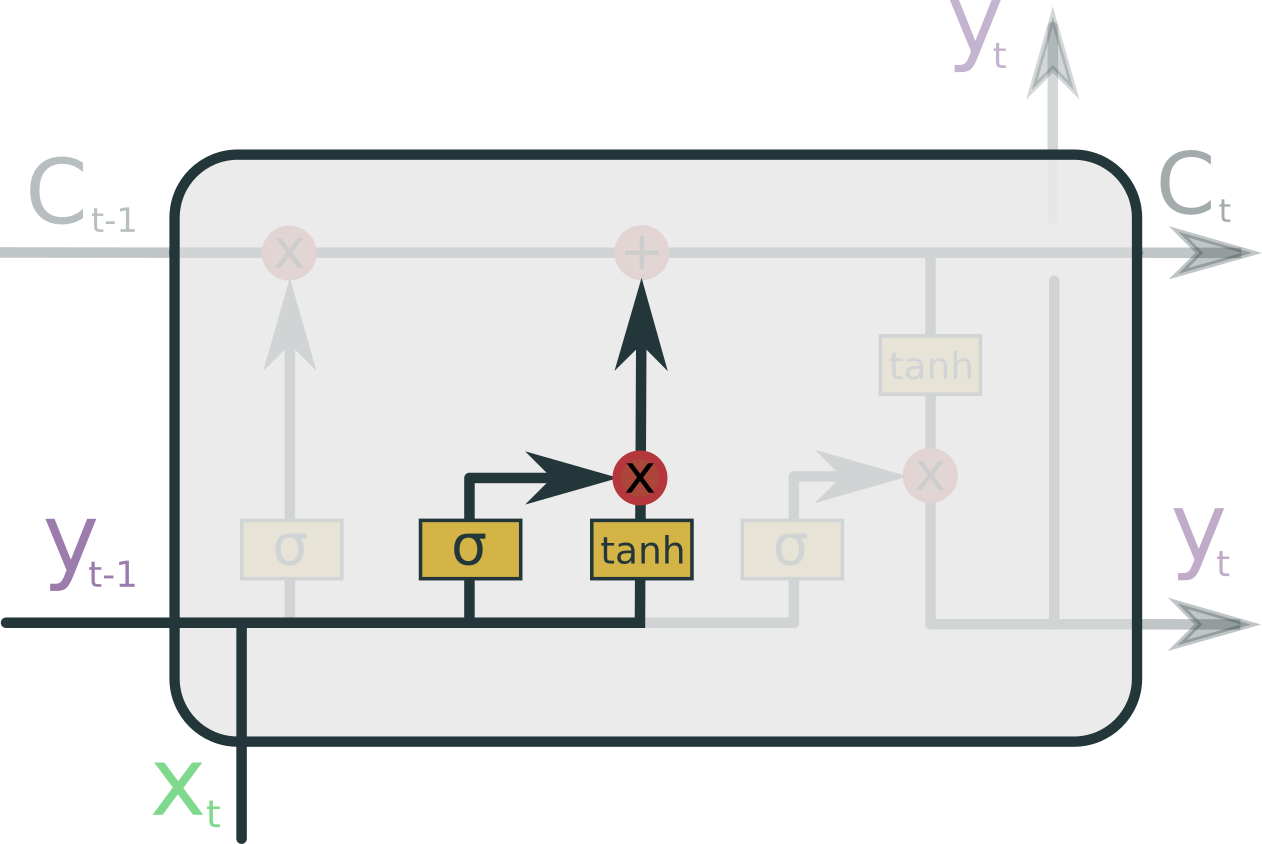
\includegraphics[width=0.5\textwidth]{images/Illustrationen/LSTM_IG}
                    \caption{Einfluss des Input Gates auf den Zellstatus (inspiriert von \cite{OLAH2015}).}
                    \label{fig:LSTM_Input}
                \end{figure}
            
            Wie der Zellstatus $C_t$ nun die Ausgabe beeinflusst, wird über das \textit{Output Gate} geregelt (siehe~\autoref{fig:LSTM_Output}).
            \begin{equation}
                \begin{split}
                    o_t &= \sigma\left(W_{oh}h_{t-1} + W_{ox}x_t + b_o \right), \\
                    h_t &= o_ttanh\left(c_t\right)
                \end{split}
            \end{equation}
            Dies soll in unserem Sprachbeispiel entscheiden, ob die Information des Genus für die Vorhersage des nächsten Wortes eine Rolle spielt. \cite{GERS2000, OLAH2015}

                \begin{figure}[ht]
                    \centering
                    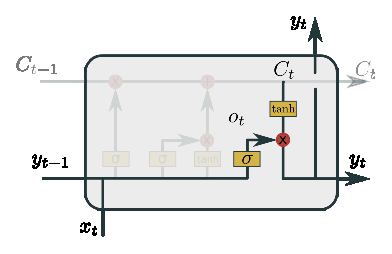
\includegraphics[width=0.5\textwidth]{images/Illustrationen/LSTM_OG}
                    \caption{Das Output Gate regelt den Einfluss des Zellstatus auf die Ausgabe des Neurons (inspiriert von \cite{OLAH2015}).}
                    \label{fig:LSTM_Output}
                \end{figure}
            
            Die verschiedenen Gates können so als ein weiteres kleines NN in jedem Knoten der LSTM Netze betrachtet werden, welche einen zeitlichen Zusammenhang besser erkennen sollen.
            Gesamt lässt sich eine LSTM Zelle mit den folgenden Formeln beschreiben:
            \begin{equation}
                \begin{split}
                    f_t &= \sigma\left(W_{fh}h_{t-1} + W_{fx}x_t + b_f\right) \\
                    i_t &= \sigma\left(W_{ih}h_{t-1} + W_{ix}x_t + b_i\right), \\
                    \tilde{C}_t &= tanh\left(W_{\tilde{C}h}h_{t-1} + W_{\tilde{C}x}x_t + b_{\tilde{C}}\right),\\
                    C_t &=f_t\times C_{t-1} + i_t\times \tilde{C}_t, \\
                    o_t &= \sigma\left(W_{oh}h_{t-1} + W_{ox}x_t + b_o \right), \\
                    h_t &= o_ttanh\left(c_t\right) \\
                    y_t &= h_t
                \end{split}
            \end{equation}
